\documentclass[tikz,border=5pt]{standalone}
\usepackage{luatexja}
\usepackage[hiragino-pron]{luatexja-preset}
\usepackage{amsmath,amssymb,bm}
\usetikzlibrary{arrows.meta,decorations.markings}

\begin{document}
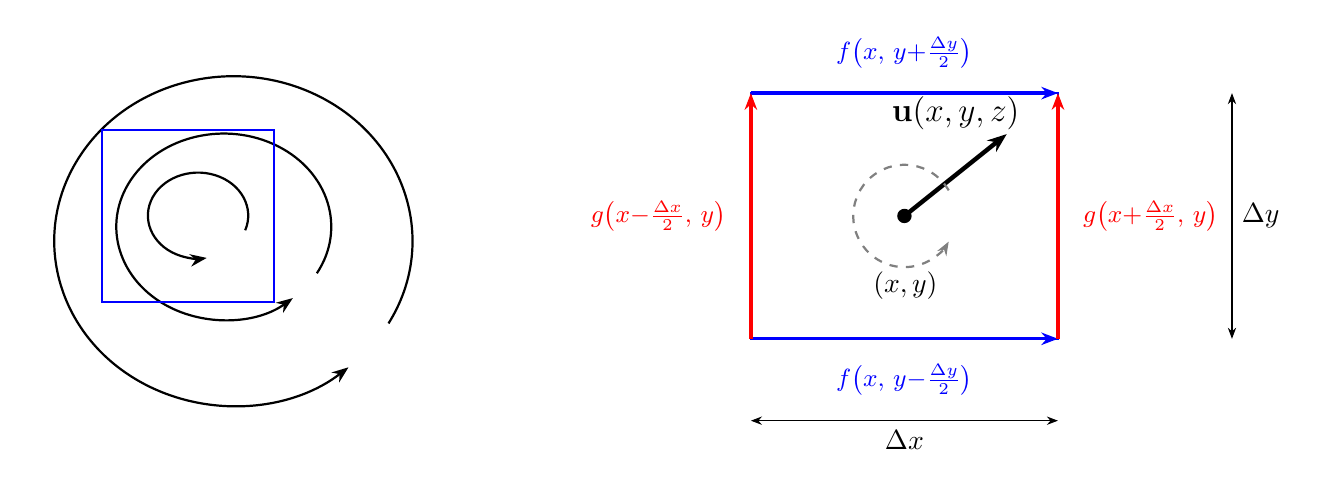
\begin{tikzpicture}[every node/.style={font=\normalsize}, scale=1.3]

  %% Left panel: spiral flow with blue rectangle
  \begin{scope}[xshift=-7cm, scale=0.7]
    % Spiral flow (counterclockwise inward)
    \draw[-{Stealth[length=6pt]}, thick]
      (2.8,-1.5) arc[start angle=-30, end angle=310, x radius=2.5, y radius=2.3];
    \draw[-{Stealth[length=6pt]}, thick]
      (1.8,-0.8) arc[start angle=-30, end angle=310, x radius=1.5, y radius=1.3];
    \draw[-{Stealth[length=6pt]}, thick]
      (0.8,-0.2) arc[start angle=-20, end angle=280, x radius=0.7, y radius=0.6];

    % Blue rectangle
    \draw[thick, blue] (-1.2,-1.2) rectangle (1.2,1.2);
  \end{scope}

  %% Right panel: detailed rectangle with circulation
  % Rectangle
  \draw[thick, blue] (-1.5,-1.2) rectangle (1.5,1.2);

  % Bottom: rightward f(x, y-Δy/2) — blue
  \draw[-{Stealth[length=6pt]}, very thick, blue] (-1.5,-1.2) -- (1.5,-1.2);
  \node[blue, below, font=\small] at (0,-1.35) {$f\!\left(x,\, y{-}\frac{\Delta y}{2}\right)$};

  % Top: rightward f(x, y+Δy/2) — blue
  \draw[-{Stealth[length=6pt]}, very thick, blue] (-1.5,1.2) -- (1.5,1.2);
  \node[blue, above, font=\small] at (0,1.35) {$f\!\left(x,\, y{+}\frac{\Delta y}{2}\right)$};

  % Right: upward g(x+Δx/2, y) — red
  \draw[-{Stealth[length=6pt]}, very thick, red] (1.5,-1.2) -- (1.5,1.2);
  \node[red, right, font=\small] at (1.65,0) {$g\!\left(x{+}\frac{\Delta x}{2},\, y\right)$};

  % Left: upward g(x-Δx/2, y) — red
  \draw[-{Stealth[length=6pt]}, very thick, red] (-1.5,-1.2) -- (-1.5,1.2);
  \node[red, left, font=\small] at (-1.65,0) {$g\!\left(x{-}\frac{\Delta x}{2},\, y\right)$};

  % Center point
  \fill (0,0) circle (2pt);
  \node[below right] at (-0.4,-0.45) {$(x,y)$};

  % Dimension labels
  \draw[{Stealth[length=4pt]}-{Stealth[length=4pt]}] (-1.5,-2.0) -- (1.5,-2.0);
  \node[below] at (0,-2.0) {$\Delta x$};

  \draw[{Stealth[length=4pt]}-{Stealth[length=4pt]}] (3.2,-1.2) -- (3.2,1.2);
  \node[right] at (3.2,0) {$\Delta y$};

  % u vector from center
  \draw[-{Stealth[length=7pt]}, ultra thick] (0,0) -- (1.0,0.8);
  \node[above, font=\large] at (0.5,0.75) {$\mathbf{u}(x,y,z)$};

  % Curved arrow for rotation sense (centered at origin)
  \draw[-{Stealth[length=5pt]}, thick, gray, dashed]
    ({0.5*cos(30)},{0.5*sin(30)}) arc[start angle=30, end angle=330, radius=0.5];
\end{tikzpicture}
\end{document}
